%%%%%%%%%%%%%%%%%%%%%%%%%%%%%%%%%%%%%%%%%%%%%%%%%%%%%%%%%%%%%%%%%%
%%%%%%%% ICML 2016 EXAMPLE LATEX SUBMISSION FILE %%%%%%%%%%%%%%%%%
%%%%%%%%%%%%%%%%%%%%%%%%%%%%%%%%%%%%%%%%%%%%%%%%%%%%%%%%%%%%%%%%%%

% Use the following line _only_ if you're still using LaTeX 2.09.
%\documentstyle[icml2016,epsf,natbib]{article}
% If you rely on Latex2e packages, like most moden people use this:
\documentclass{article}

% use Times
\usepackage{times}
% For figures
\usepackage{graphicx} % more modern
%\usepackage{epsfig} % less modern
\usepackage{subfigure} 

% For citations
\usepackage{natbib}

% For algorithms
\usepackage{algorithm}
\usepackage{algorithmic}

% For equations
\usepackage{amsmath}
\usepackage{amsfonts}


% As of 2011, we use the hyperref package to produce hyperlinks in the
% resulting PDF.  If this breaks your system, please commend out the
% following usepackage line and replace \usepackage{icml2016} with
% \usepackage[nohyperref]{icml2016} above.
\usepackage{hyperref}

% Packages hyperref and algorithmic misbehave sometimes.  We can fix
% this with the following command.
\newcommand{\theHalgorithm}{\arabic{algorithm}}

% Employ the following version of the ``usepackage'' statement for
% submitting the draft version of the paper for review.  This will set
% the note in the first column to ``Under review.  Do not distribute.''
\usepackage[accepted]{icml2016} 

\usepackage{csvsimple}

% Employ this version of the ``usepackage'' statement after the paper has
% been accepted, when creating the final version.  This will set the
% note in the first column to ``Proceedings of the...''
%\usepackage[accepted]{icml2016}


% The \icmltitle you define below is probably too long as a header.
% Therefore, a short form for the running title is supplied here:
\icmltitlerunning{Review of Frank Wolfe and its variants}

\begin{document} 

\twocolumn[
\icmltitle{Review of Frank Wolfe and its variants}

% It is OKAY to include author information, even for blind
% submissions: the style file will automatically remove it for you
% unless you've provided the [accepted] option to the icml2016
% package.
\icmlauthor{William Saint-Arnaud}{william.st-arnaud@umontreal.ca}
\icmlauthor{Elyes Lamouchi}{elyeslamouchi@gmail.com}
\icmlauthor{Frederic Boileau}{frederic.boileau@umontreal.ca}


% You may provide any keywords that you 
% find helpful for describing your paper; these are used to populate 
% the "keywords" metadata in the PDF but will not be shown in the document
% \icmlkeywords{boring formatting information, machine learning, ICML}

\vskip 0.3in
]
\begin{abstract} 
Due to the combinatorial nature of multilabel outputs, predicting structured data typically comes with an exponentially large number of constraints, which makes the problem inefficient or intractable in practice. There has been a lot of research focused on providing a solution to that issue. In the structured SVM setting, conditional gradient a.k.a  Frank-Wolfe type algorithms have become a method of choice.\\
\\
This paper's aim is to synthesize the recent advances, starting from the classical F-W to the more sophisticated variants, while motivating this with the problems each variant addresses. Finally, we will discuss the pitfalls of some variants and their intrinsic trade-offs. 
We will then evaluate the performance of the methods proposed on synthetic data to see how reasonable the assumptions (providing theoretical guarantees)are, and to get an idea whether each variant's trade-off is worth it.
\end{abstract} 
\section{Extragradient Algorithm for structured predictions}
\subsection{Preliminaries}
In the typical setting for SVM's, we aim to optimize a linear objective over a
set of constraints. There are many alernatives to solve that problem, the most
popular ones being gradient-based methods. One of the issues with this type of
algorithm is that they cannot be applied to matchings and min-cuts. In addition,
variants that aim at generating constraints on the fly and incrementally solving
new QP's do not typically scale well. The method proposed in this paper, which
is in essence a modification of the extra-gradient method by Nesterov, leverages
the min-max formulation and takes the dua ; the exponential number of
constraints in then transformed an exponential number of variables. However, the
paper highlights that we can use only a tractable number of these dual variables
to solve the optimization problem. The method prososed in this paper also
generalizes the applicability of the usual extra-gradient method to
non-euclidean, Bergman projections. We thus end up with a framework that is more
flexible and also efficient to implememt.

Since estimating the maximum likelihood over graphical models is often
impractical or infeasible for a wide class of problems, we focus our attention
on large margin estimation. For a dataset $ S = \{ (\vec x_i, \vec y_i) \}_{i=1}^{m} $,
where each $\vec x_i$ is an object with a structure (e.g. sequence of words in
french), we attempt to find the optimal parameter $\vec w$ of a linear classifier:

\begin{equation}
  \vec y_i = \argmax_{\vec y_i' \in \mathcal{Y}} \vec w^T \vec f(\vec x_i,\vec y_i')
  \label{eq1}
\end{equation}

The function $f$ gives a feature mapping of a structured object with its
corresponding label $\vec y_i$. The error of a prediction is mesured by a loss
function $l$. To make the loss convex, another term is introduced in the form a
hinge loss. Since this gives an upper bound to the loss, it is natural to
minimize it. We end up with a problem of the form:

\begin{equation}
  \min_{\vec w \in \mathcal{W}} \sum_i \max_{\vec y_i' \in \mathcal{Y}_i} \left[
\vec w^T \vec f_i(\vec y_i') + l_i(\vec y_i') \right] - \vec w^T \vec f_i(\vec
y_i)
\end{equation}

The parameters $\vec w$ are also regularized with parameter $\lambda$. Since we are
optimizing over $\vec y_i'$, we can drop the term from equation \ref{eq1} and we end
up with a loss-augmented inference problem inside the min function. The three
types of structure that are presented in the paper have a general formulation
that can better be expressed as:

\begin{equation}
  \min_{\vec w \in \mathcal{W}} \max_{\vec z \in \mathcal{Z}} \sum_i \left( \vec
w^T \vec F_i \vec z_i + \vec c_i^T \vec z_i - \vec w^T \vec f_i(\vec y_i)
\right)
  \label{saddle_point}
\end{equation}

where the $\vec z_i$'s can be identified with the edge and node potentials of a
markov network and satisfy the constraints of the structured problem. The terms
$\vec F_i$ correspond to the feature mapping for over all labels $\vec y_i$ when
multiplied by $\vec z_i$'s. The $\vec c_i$'s correspond to the costs of a $\vec z_i$ and can be
identified with the loss $l$ for a label $\vec y_i'$. Taking the dual, we end up with
the following:

\begin{equation}
  \begin{aligned}
    &\min_{\vec w \in \mathcal{W}, (\vec \lambda,\vec \mu) \geq \vec 0} &\sum_i
\left( \vec b_i^T \lambda_i + \mathbf{1}^T \vec \mu_i - \vec w^T \vec f_i(\vec
y_i) \right)\\ &\text{s.t.} &\vec F_i^T \vec w + \vec c_i \leq \vec A_i^T \vec
\lambda_i + \vec \mu_i \quad i=1,\dots,m
  \end{aligned}
\end{equation}

The number of variables and constraints is linear in the number of paramters and
training data. We already see that this formulation is much more efficient. We
do have a set of constraints that is tractable, as is the number of parameters
to update. In equation \ref{saddle_point}, the term that is opitmized is defined
as:

\begin{equation}
  \mathcal{L}(\vec w,\vec z) \triangleq \sum_i \vec w^T \vec F_i \vec z_i + \vec
c_i^T - \vec w^T \vec f_i(\vec y_i)
  \label{saddle_obj}
\end{equation}

It is bilinear in $w$ and $z$. We can then imagine two players represented by
$\vec w$ and $\vec z$ that play a zero-sum game. They perform updates using gradients of
the objective w.r.t. their parameters. They then project the result to the set
of feasible points given by the constraints imposed on the structure. We usually
consider Euclidean projections, as there are well-known problems where they are
efficient to compute. However, as seen later, this is not the case for all
problem. This is why Bregman projections will be introduced. Going back to the
zero-sum game, we have the following operator that is used to perform the
updates for both players at the same time.

\begin{equation*}
 &\textit{Let}\quad\vec F= \begin{pmatrix}
 \begin{array}{cccc}
    0 & \vec F_1 & \dots & \vec F_m\\
    -\vec F_1^T & & &\\
    \vdots & & \vec 0 &\\
    -\vec F_m^T & & &
 \end{array}
\end{pmatrix}
\end{equation*}
\begin{equation*}
 &\vec u= \begin{pmatrix}
      \begin{array}{c}
        \vec w\\
        \vec z_1\\
        \vdots\\
        \vec z_m
      \end{array}
    \end{pmatrix}\quad\textit{and}\quad
 &\vec a=  \begin{pmatrix}
      \begin{array}{c}
        \sum_i \vec f_i(\vec y_i)\\
        \vec c_1\\
        \vdots\\
        \vec c_m
      \end{array}
    \end{pmatrix}
\end{equation*}
\begin{equation*}
 &\textit{ such that }\begin{pmatrix}
    \begin{array}{c}
      \nabla_{\vec w} \mathcal{L}(\vec w,\vec z)\\
      -\nabla_{\vec z_1} \mathcal{L}(\vec w,\vec z)\\
      \vdots\\
      -\nabla_{\vec z_m} \mathcal{L}(\vec w,\vec z)
    \end{array}
  \end{pmatrix} = \vec F \vec u - \vec a
\end{equation*}


We can measure the ``goodness'' of the parameters using the gap function
$\mathcal{G}$:
\begin{equation}
  \mathcal{G}(\vec w, \vec z) \triangleq \left[ \max_{\vec z' \in \mathcal{Z}}
\mathcal{L}(\vec w,\vec z') - \mathcal{L}^* \right] + \left[ \mathcal{L}^* -
\min_{\vec w' \in \mathcal{W}} \mathcal{L}(\vec w', \vec z) \right]
\end{equation}

where $\mathcal{L}^*$ gives the result of the min-max of the objective
$\mathcal{L}$. When we have a non-optimal point (i.e. not a saddle point), the
gap is strictly positive. At at an optimal point, the gap is exaclty equal to 0.
Now the restricted gap is exactly the same but the min and max are computed over
a set of parameters that are within a certain distance of the start point
$(\hat{\vec u}_{\vec w},\hat{\vec u}_{\vec z}) \in \mathcal{U}$:
\begin{equation}
\begin{aligned}
    &\mathcal{G}_{D_{\vec w}, D_{\vec z}}(\vec w, \vec z) = \max_{\vec z' \in \mathcal{Z}} \left[ \mathcal{L}(\vec w', \vec z') : d(\vec z, \vec z') \leq D_{\vec z} \right]\\
    &\quad\quad\quad\quad-\left [ \min_{\vec w' \in \mathcal{W}} \mathcal{L}(\vec w',\vec z) : d(\vec w, \vec w') \leq D_{\vec w'} \right ]
\end{aligned}
\end{equation}

The motivation for using this restricted gap function is that if we start ``close'' to an optimal point, of course we will converge more rapidly to it. This can be seen in the convergence analysis of the method. 

\subsection{Dual Extragradient algorithm}

The dual extragradient algorithm from Nesterov gives a convergence guarantee for the objective $\mathcal{L}$. The algorithm can be given by:
\begin{algorithm}[tb]
   \caption{Dual Extragradient}
   \label{alg:example}
\begin{algorithmic}
  \STATE Initialize: Choose $\hat{\vec u} \in \mathcal{U}$, set $\vec s^{-1} = 0$.
  \FOR{$t=0$ to $t=\tau$} 
  \STATE $\vec v = \mathbf{\Pi}_{\mathcal{U}}(\hat{\vec u} + \eta \vec s^{t-1})$\\
  \STATE $\vec u^t = \mathbf{\Pi}_{\mathcal{U}}(\vec v - \eta (\vec F \vec v - \vec a))$\\
  \STATE $\vec s^t =  \vec s^{t-1} - (\vec F \vec u^t - \vec a)$
  \ENDFOR\\
  \STATE \textbf{return} $\overline{\vec u^{\tau}} = \frac{1}{1 + \tau} \sum_{t=0}^{\tau} \vec u^t$
\end{algorithmic}
\end{algorithm}

This algorithm has a lookahead step (i.e. $v$) that serves the peform the actual
gradient update $u^t$. The intuition behind the lookahead step is that given a
function to optimize that is Lipschitz, Nesterov was able to show that we can
upper bound $f_{D}(\bar{u^n}) = \max_y \left \{ \langle g(y),\bar{u^n} - y
\rangle : d(\hat{u},y) \leq D \right \}$, where $\bar{u^n}$ is the weighted
average over all the updates $u^t$ up to iteration n. The function g corresponds
to the objective $\mathcal{L}$ in our setting. When value of $f_D(\bar{u^n})$
gets close to 0, we have that the value $g(y^*)$ for an optimal $y^*$ is close
to 0, which signifies that we have reached saddle point (i.e. what we wanted).
Nesterov goes on to show that this upper bound indeed goes to 0. We then get
convergence to a saddle point. Note that in the definition of $f_D$, we used a
distance metric d. This corresponds to the Euclidean distance (or Bregman
distance in non-Euclidean setting). The rojection operator $\Pi_{\mathcal{U}}$
in the algorithm simply projects a point back to the set $\mathcal{U}$ by
finding the nearest point with respect to the distance metric used.
\subsubsection{Proximal step operator}
We define the proximal step operator as follows:
\begin{equation}
  \mathcal{T}_{\eta}(\vec u, \vec s) = \max_{\vec u \in \mathcal{U}} \left \{ \langle \vec s, \vec u' - \vec u \rangle - \frac{1}{\eta}  d(\vec u, \vec u') \leq D \right \}
\end{equation}

The operator is useful to compute projections since when we have a strongly convex function $h(\vec u)$, we can find its convex conjugate $h^*(\vec u) = \max_{\vec u  \in \mathcal{U}} \left [ \langle \vec s, \vec u \rangle - h(\vec u) \right ]$. From the definition of a strongly convex function, we have that:
\begin{equation}
  h(\vec u') \geq h(\vec u) + \langle \nabla h(\vec u), \vec u'  - \vec u \rangle + \frac{\sigma}{2} \lVert \vec u' - \vec u \rVert^2
\end{equation}
where $\sigma$ is the strong convexity parameter. Rearranging, we can define an upper bound on the squared norm of $\vec u' - \vec u$. This comes out as:
\begin{equation}
  d(\vec u', \vec u) \triangleq h(\vec u') - h(\vec u) - \langle \nabla h(\vec u), \vec u' - \vec u \rangle \geq \frac{\sigma}{2} \lVert \vec u' - \vec u \rVert^2
\end{equation}

The distance metric $d$ is called the Bregman divergence. The link between the Bregman diverence and the proximal step operator is that if we are given the function $h$ inside the definition of the proximal step update, this induces the Bregman divergence, which in turn induces the update that is performed at each iteration of the extragradient algorithm. For example, if we have $h(\vec u) = \frac{1}{2} \lVert \vec u \rVert_2^2 $, the Bregman divergence becomes $d(\vec u', \vec u) = \frac{1}{2} \lVert \vec u' - \vec u' \rVert_2^2$. We might wonder why we care about the Bregman divergence when the definition still includes the usual norm. After all, we still optimize the term $\langle \vec s, \vec u' - \vec u \rangle - \frac{1}{\eta} d(\vec u', \vec  u)$. This is because $h*$ is differentiable at every point of its domain by the strong convexity of $h$. Thus, it is easy to compute a projection in the usual fashion: we can compute the derivative of the termn inside the projection operator and set it to 0. It is impossible to do for matchings for example as the distance is not even differentiable. We provide the steps to compute a projection: 
\begin{equation}
\begin{aligned}
  &\vec s - \nabla_{\vec u'} d(\vec u', \vec u) = \vec s - \frac{1}{\eta} \nabla_{\vec u'} d(\vec u, \vec u')\\
  &= \vec s - \frac{1}{\eta} \left [\nabla h(\vec u') - \nabla h(\vec u) \right]
\end{aligned}
\end{equation}

By setting this equation to 0, it is possible to recover the optimal $\vec y'$ when, let's say, $h(\vec u) = \frac{1}{2} \lVert \vec u' \rVert^2$. 

\subsubsection{Convergence analysis} 
The restricted gap function
$\mathcal{G}_{D_{\vec v}, D_{\vec z}}$ is upper bounded by:
\begin{equation} \mathcal{G}_{D_{\vec w}, D_{\vec z}}(\overline{\vec w^{\tau}},
\overline{\vec z^{\tau}}) \leq \frac{\left( D_{\vec w} + D_{\vec z} \right)
L}{\tau + 1}
\label{eq:ub}
\end{equation}

In his proof on the convergence of the extragradient algorithm, Nesterov uses a
function $f_D$ instead of $\mathcal{G}_{D_{\vec w}, D_{\vec z}}$, where $f_D$ is
defined as:
\begin{equation}
f_D(\vec x) = \max_{\vec y \in \mathcal{Q}} \left \{ \langle g(\vec y), \vec x -
\vec y \rangle : d(\vec x, \vec y) \right \}
\end{equation}

where the set $\mathcal{Q}$ is the set of parameters and $g$ is a monotone
operator. We can already see a link between the function $f_D$ and the gap
$\mathcal{G}_{D_{\vec w}, D_{\vec z}}$. This comes out as:

\begin{equation}
  \begin{aligned}
    &\mathcal{G}_{D_{\vec w},D_{\vec z}}(\vec w, \vec z) = \sum_i \vec w^T \vec F_i \vec z_i^* - (\vec w^*)^T \vec F_i \vec z_i - \sum_i (\vec w^T - (\vec w^*)^T ) \vec f_i (\vec y_i)\\
    &\quad\quad\quad\quad- \sum_i \vec c_i^T (\vec z_i - \vec z_i^*)\\
    &= \sum_i (\vec z_i^*)^T \vec F_i^T \vec w - (\vec w^*)^T \vec F_i \vec z_i - \sum_i \vec (\vec f_i (\vec y_i))^T (\vec w - \vec w^*)\\
    &\quad\quad\quad\quad- \sum_i \vec c_i^T (\vec z_i - \vec z_i^*)\\
    &= \sum_i (\vec z_i^*)^T \vec F_i^T (\vec w - \vec w^*) - (\vec w^*)^T \vec F_i (\vec z_i - \vec z_i^*)\\
    &\quad\quad\quad\quad- \sum_i (\vec f_i(\vec y_i))^T (\vec w - \vec w^*) - \sum_i \vec c_i^T (\vec z_i - \vec z_i^*)\\
    &=  
    \begin{pmatrix}
      \begin{array}{c}
        \sum_i \vec F_i \vec z_i^*\\
	-\vec F_1^T \vec w^*\\
	\vdots\\
	-\vec F_m^T \vec w^*
      \end{array}
    \end{pmatrix}^T 
    \begin{pmatrix}
      \begin{array}{c}
	\vec w - \vec w^*\\
	\vec z_1 - \vec z_1^*\\
	\vdots\\
	\vec z_m - \vec z_m^*
      \end{array}
    \end{pmatrix} - 
    \begin{pmatrix}
      \begin{array}{c}
	\sum_i \vec f_i(\vec y_i)\\
	\vec c_1\\
	\vdots\\
	\vec c_m
      \end{array}
    \end{pmatrix}^T
    \begin{pmatrix}
      \begin{array}{c}
	\vec w - \vec w^*\\
	\vec z_1 - \vec z_1^*\\
	\vdots\\
	\vec z_m - \vec z_m^*
      \end{array}
    \end{pmatrix}
  \end{aligned}
\end{equation}

From this, we deduce that the function $g$ from the definition of $f_D$ corresponds to:
\begin{equation}
  g(\vec w, \vec z) =
  \begin{pmatrix}
    \begin{array}{c}
      \sum_i \vec F_i \vec z_i^*\\
      - \vec F_i^T \vec w^*\\
      \vdots\\
      - \vec F_m^T \vec w^*
    \end{array}
  \end{pmatrix} -
  \begin{pmatrix}
    \begin{array}{c}
      \sum_i \vec f_i (\vec y_i)\\
      \vec c_1\\
      \vdots\\
      \vec c_m
    \end{array}
  \end{pmatrix} = \vec F \vec u^* - \vec a
\end{equation}
It is constant and thus monotone as required by Nesterov's proof of the convergence of the algorithm. Its Lipschitz constant $L$ is equal to $\max_{\vec u \in \mathcal{U}} \lVert \vec F (\vec u - \vec u') \rVert_2 / \lVert \vec u - \vec u' \rVert_2 \leq \lVert \vec F \rVert_2$. Of course, a point $\vec w, \vec z$ that satisifies $\lVert \vec w \rVert_2 \leq D_{\vec w}$ and $\lVert \vec z \rVert_2 \leq D_{\vec z}$ also satisifies $\lVert (\vec w, \vec z) \rVert_2 \leq D$ when $D = \sqrt{D_{\vec w}^2 + D_{\vec z}^2}$ since $(\vec w, 0) \perp (0, \vec z)$. It is then easy to see that $f_D \geq \mathcal{G}_{D_{\vec w}, D_{\vec z}}$. Thus, the function $\mathcal{G}_{D_{\vec w}, D_{\vec z}}$ is upper bounded by the right-hand side of equation \ref{eq:ub}. We can also observe that the function $g(\vec w, \vec z)$ is exactly the gradient of the objective $\mathcal{L}(\vec w, \vec z)$ at the point $\vec w, \vec z$.


\subsection{Non-Euclidean setting}
The main problem with the Euclidean projection operator is that for many
problems, it is hard to compute the projection. Indeed for min-cut, we need to
compute the partition function first, which is \#P-complete. Thus, the authors
of the paper introduced the Bregman operator, which computes the projection
using the Bregmand divergence. Using this operator has the great advantage of
being easier to compute. We can see this for $L1$ regularization. Computing a
projection using $L1$ distance is hard since it is not differentiable. Using the
negative entropy, we get that the Bregman divergence is the KL divergence. This
implies that we can differentiate the divergence to get the parameter that
minimizes it.

\subsection{Memory-efficient tweak}
In the dual extragradient algorithm, both a vector $s^t$ and a vector
$\bar{u^t}$ are maintained. However, we can observe that the $s_t$'s can be
found using the running average $\bar{u^t}$ since $s^t = -(t + 1 ) \sum_{i=0}^t
(F \bar{u^t} - a)$. We only have to store the vector $\bar{u^t}$. We can even do
better when $|\mathcal{Z}| \gg |\mathcal{W}|$ since $\bar{u^t} = \{
\bar{u^t}_w,\bar{u^t}_z \}$ and we only care about the part that corresponds to
$w$. $\bar{u^t}_z$ is maintained implicitly by storing a vector of size
$|\mathcal{W}|$ (although we now need to store $s_w^t$). It can be reconstructed
using $\bar{u^t}_w$. Figure 1 illustrates the various dependencies.

\begin{figure}
  \includegraphics[width=\linewidth]{fig5.png}
  \caption{Dependency diagram for memory-efficient dual extragradient. The dotted box represents the computations of an iteration of the algorithm.}
  \label{fig:Dependency diagram}
\end{figure}


%%%%%%%%%%%%%%%%%       FRANK WOLFE
\section{From classical Frank-Wolfe to more sophisticated variants}
\subsection{Classical Frank-Wolfe}
Consider the problem of minimizing a convex objective function $f$ over the convex hull of its domain $\mathcal{M}= conv(\mathcal{A})$.\\
By minimizing the first-order approximation of the objective function, the Frank-Wolfe algorithms takes a convex combination of the immediate iterate with the previous one. Consider a linear minimization oracle,
\begin{equation*}
\begin{aligned}
    &LMO_{\mathcal{A}}(\nabla f(x_{t}))\in \textit{argmin}_{s\prime\in\mathcal{A}}\langle s\prime, \nabla f(x_{t})\rangle
\end{aligned}    
\end{equation*}
Starting with an active set consisting of only an initial feasible point $S^{0}= \{x_{0}\}$, the Frank-Wolfe algorithm adds an "atom" $s_{t}= LMO_{\mathcal{A}}(\nabla f(x_{t}))$, to the active set in a convex combination with its elements while maintaining this combination sparse.
\subsubsection{Convergence results}
We define the duality gap
\begin{equation*}
\begin{aligned}
    &g(\alpha^{k})= \underset{s\in\mathcal{M}}{\textit{max}}\langle \alpha^{k}-s, \nabla f(\alpha^{k})\rangle
\end{aligned}
\end{equation*}
By first order convexity of the objective, we have
\begin{equation*}
\begin{aligned}
    &f(s)\geq f(\alpha^{k})+ \langle \alpha^{k}-s, \nabla f(\alpha^{k})\rangle\\
    &\Longrightarrow g(\alpha^{k})= -\underset{s\in\mathcal{M}}{\textit{min}}\langle \alpha^{k}-s, \nabla f(\alpha^{k})\rangle \geq f(\alpha^{k})- f^{*}
\end{aligned}
\end{equation*}
We can thus see that the duality gap gives us a computable optimality guarantee. 
\\
\\
\textbf{Definition.} The curvature constant $C_{f}$ is given by the maximum relative deviation of the objective function f from its linear aaporximations, over the domain $\mathcal{M}$,
\begin{equation*}
\begin{aligned}
    &C_{f}= \underset{\underset{ \gamma\in[0,1], y=x+\gamma(s-x)}{x,s\in\mathcal{M}}}{sup}\frac{2}{\gamma^{2}}\Big(f(y)- f(x)- \langle y-x, \nabla f(x)\rangle\Big)
\end{aligned}
\end{equation*}
\\
Intuitively, the curvature constant can be seen as a measure of how flat the objective function is. For example, if the objective is linear, say $f(x)= ax+ b$ and $x\in[e,f]$ then $\nabla f(x)= a$ and the curvature constant is zero:
\begin{equation*}
\begin{aligned}
    &C_{f}= \frac{2}{\gamma^{2}}\Big(ay+ b- ax- b +(-ay +ax)\Big)= 0
\end{aligned}
\end{equation*}
Moreover $s=\textit{argmin}_{s\in[e,f]}\langle s, a\rangle= \frac{e}{a}$. Hence we reach the minimum in one F-W step.\\
Thus, we can observe that for flatter functions, that is with smaller curvature constants, Frank-Wolfe should converge faster.
\\
\\
\textbf{Theorem.} The duality gap obtained in the $t^{th}$  iteraton of the Frank-Wolfe algorithm satisfies
\begin{equation*}
\begin{aligned}
    &g(x_{t})\leq 2\beta\frac{C_{f}}{t+2}(1+\delta)
\end{aligned}
\end{equation*}
Where $\beta= \frac{27}{8}$ and $\delta$ is the approximation error tolerated in the $LMO$.
\\
\\
\textbf{Definition.} A function $f$ has Lipschitz continuous gradient if: 
\begin{equation*}
\begin{aligned}
    &\forall x,y \in dom(f), \exists L >0 \quad\textit{such that}\quad\\
    &||\nabla f(x) -\nabla f(y)||^2 \leq L||x - y||^2
\end{aligned}
\end{equation*}
\textbf{Theorem.} If a convex function $f$ on $C$ has Lipschitz gradient, i.e $||\nabla f(x)- \nabla f(y)||_{p}\leq L_{q}||x- y||_{p},\quad\forall x,y\in C$, then
\begin{equation*}
\begin{aligned}
      &C_{f}\leq L_{q}.\text{diam}_{p}^{2}(C)
\end{aligned}
\end{equation*}
\\
\textbf{\textit{Proof.}} $f$ has Lipschitz gradient therefore by the fundamental descent lemma we have,
\begin{equation*}
\begin{aligned}
      &f(y)- f(x)- \langle y- x, \nabla f(x)\rangle \leq \frac{L_{q}}{2}||y- x||_{p}^{2}\\
      &C_{f} \leq \underset{\underset{x,s,y\in C}{y=(1-\gamma)x+\gamma s}}{max}\frac{2}{\gamma^{2}}\frac{L_{q}}{2}\underbrace{||y- x||_{p}^{2}}_{=\gamma^{2}||x- s||_{p}^{2}}\\
      &C_{f} \leq L_{q}\quad\underbrace{\underset{x,s\in C}{max}||x- s||_{p}^{2}}_{\overset{\Delta}{=}\textit{diam}_{p}^{2}(C)}\quad\quad\Box.
\end{aligned}    
\end{equation*}
Therefore, assuming $\delta=0$, we get the following optimality certificate
\begin{equation*}
\begin{aligned}
      &f(\alpha^{k})- f^{*}\leq  g(\alpha^{k})\leq 2\beta\frac{C_{f}}{t+2}\leq 2\beta\frac{L_{q}.\text{diam}_{p}^{2}(C)}{t+2}
\end{aligned}    
\end{equation*}
Thus, we see that the Frank-Wolfe algorithm has a sublinear convergence rate.
\subsubsection{Optimality in terms of sparsity of the iterates}
\textbf{Lemma.} For $f(x)= ||x||_{2}^{2}$ and $1\leq k\leq n$, it holds that
\begin{equation*}
\begin{aligned}
      &\textit{min}_{\underset{card(x)\leq
      k}{x\in\Dalta_{n}}}f(x)= \frac{1}{k},\quad\textit{and}\\
      &g(x)\geq \frac{2}{k}\quad\forall x\in\Delta_{n}\quad\textit{s.t.}\quad card(x)\leq k. 
\end{aligned}    
\end{equation*}
By the first equality we have, for any vector $x$ s.t. $card(x)= k$, we get $g(x)\leq \frac{1}{k}- \frac{1}{n}$.
Thus, combining the upper and lower bound, we have that the sparsity (number of used atoms) by the Frank-Wolfe algorithm is worst case optimal.
\begin{algorithm}[tb]
   \caption{Frank-Wolfe}
   \label{alg:example}
\begin{algorithmic}
   \STATE Let $\alpha\in\mathcal{M}$
   \FOR{$k=0$ {\bfseries to} $K$}
   \STATE {Compute $s={\textit{argmin}}_{s\in\mathcal{M}}\langle s, \nabla f(\alpha^{k})\rangle$}
   \STATE Let $\gamma = \frac{2}{k+2}$, or optimize $\gamma$ by line search
   \STATE Update $\alpha^{k+1}= (1-\gamma)\alpha^{k}+ \gamma s$
   \ENDFOR
\end{algorithmic}
\end{algorithm}
\subsection{Away steps Frank-Wolfe}
When the minimizer of the objective function lies at the boundary of the domain, after a number of iterations, the duality gap starts to stagnate.\\
As a result of the strong dependency of the immediate iterate on previously accumulated atoms in the active set, as it approaches to boundary, the F-W algorithm starts to zig-zag around the descent direction as can be seen in figure 2.\\
\begin{algorithm}[tb]
   \caption{Away-steps Frank-Wolfe}
   \label{alg:example}
\begin{algorithmic}
    \STATE {Let $x_{0}\in\mathcal{A}$ and $S_{0}:=\{x_{0}\}$}\\
    \FOR {$t=0...T$}{
        \STATE{Let $s_{t}:= LMO_{\mathcal{A}}(\nabla f(x_{t}))$ and $d^{FW}_{t}:= s_{t}- x_{t}$}\\
        \STATE{Let $v_{t}\in \underset{v\in S_{t}}{\textit{argmax}}\langle\nabla f(x_{t}), v\rangle$ and $d^{A}_{t}:= x_{t}- v_{t}$}\\
        \STATE {\textbf{if} $g^{FW}_{t}=\langle-\nabla f(x_{t}), d^{FW}_{t}\rangle\leq \epsilon$ \textbf{then return} $x_{t}$}\\
        \STATE {\textbf{if} $\langle-\nabla f(x_{t}), d^{FW}_{t}\rangle\geq \langle-\nabla f(x_{t}), d^{A}_{t}\rangle$\quad\textbf{then}}\\ \STATE{\quad\quad\quad$d_{t}=d^{FW}_{t}$ and $\gamma^{max}=1$}\\
        \STATE{\textbf{else}}\\
        \STATE{\quad\quad\quad $d_{t}=d^{A}_{t}$ and $\gamma^{max}=\frac{\alpha^{(t)}_{v_{t}}}{1-\alpha^{(t)}_{v_{t}}}$}\\
        \STATE{Line-search: $\gamma_{t}\in\underset{\gamma}{argmin}f(x_{t}+\gamma d_{t})$}\\
        \STATE{Update $x_{t}= x_{t}+\gamma_{t}d_{t}$}\\
    }
    \ENDFOR
\end{algorithmic}
\end{algorithm}
\begin{figure}
  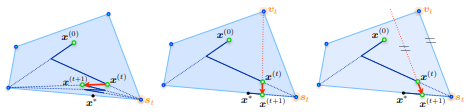
\includegraphics[width=\linewidth]{fig2.png}
  \caption{(left) The FW algorithm zig-zags when the solution $x$ lies on the boundary. (middle) Adding the possibility of an away step attenuates this problem. (right) As an alternative, a pairwise FW step.}
  \label{fig:Away steps}
\end{figure}
\\
To address this issue an improved variant of F-W named \textbf{Away-steps Frank-Wolfe} adds the possibility of moving away (by removing a fraction of) a maximizer of the $LMO_{\mathcal{S_{t}}}$ in the active set. While this slows down each iteration it should be noted that the added step is easier than $LMO_{\mathcal{A}}$ given that we maximize over a subset of $\mathcal{A}$. Furthermore, given that this variant converges linearly, the algorithm progresses in a fewer number of iterations in the descent direction, making it much faster than the original F-W.
\subsection{Block Coordinate Frank Wolfe}
\subsubsection{Structured SVM context}
Given a training set $\mathcal{D}=\{(x_i,y_i)\}_{i=1}^n$ where $y \in \mathcal{Y}$ is a multi-label output, and a feature map $\phi:\mathcal{X}\times\mathcal{Y}\longrightarrow \mathbb{R}$, which encodes a similarity measure between $\mathcal{X}$ and $\mathcal{Y}$, such that if $y_{i}$ is the ground truth (target) for an input $x_{i}$, then
\begin{equation*}
\begin{aligned}
    &\forall y\in\mathcal{Y}\texttt{\symbol{92}}\{y_{i}\}\quad\textit{we have}\quad \psi_{i}(y) = \phi(x_{i},y_{i})- \phi(x_{i},y) > 0
\end{aligned}
\end{equation*}
The aim is to construct an accurate linear classifyer, $h_{w}(x)= \underset{y\in\mathcal{Y}(x)}{\textit{argmax}}\langle w, \phi(x,y)\rangle$.\\
To learn $w$, consider the task loss $L:\mathcal{Y}\times\mathcal{Y}\longrightarrow\mathbb{R}_{+}$, where $L(y,y\prime)= 0 \Longleftrightarrow y= y\prime$.
\\
The $n$-slack formulation of the problem would be,
\begin{equation*}
\begin{aligned}
    &\underset{w,\xi}{\textit{max}}\quad\frac{\lambda}{2}||w||^{2}+ \frac{1}{n}\sum_{i=1}^{n}\varepsilon_{i}\\
    &\textit{s.t.}\quad \langle w, \psi_{i}(y)\rangle \geq L(y_{i},y)- \varepsilon_{i},\quad\forall i ,\forall y\in\mathcal{Y}(x)=\mathcal{Y}_{i}
\end{aligned}
\end{equation*}
\textit{Problems:} (1) The zero-one loss is not differentiable and (2) we have an exponential number of constraints.\\
\textit{Solutions:} (1) Minimizing an upper bound to the task loss gives us a worst case guarantee.
\\
\\
Consider the \textbf{max oracle}, $\Tilde{H}= \underset{y\in\mathcal{Y}_{i}}{\textit{max}}$ $\underbrace{L_{i}(y)- \langle w, \psi_{i}(y)\rangle}_{= H_{i}(y,w)\quad\textit{the hinge loss}}$.\\
(2) The exponential number of constraints are replaced by $n$ piecewise linear ones.
\\
\\
\textbf{Proposition.} The max oracle is a convex upper bound to the task loss.\\
\textit{Proof.} The maximum of two convex (linear) functions is convex, and
\begin{equation*}
\begin{aligned}
    &L(y_{i},h_{w}(x_{i})) \leq L(y_{i},h_{w}(x_{i})) + \underbrace{\langle w, \psi_{i}(y)\rangle}_{\geq 0 \textit{ by definition}} \\
    &\quad\quad\leq \underset{y\in\mathcal{Y}_{i}}{\textit{max}} L_{i}(y)- \langle w, \psi_{i}(y)\rangle
\end{aligned}
\end{equation*}
Thus learning $w$ amounts to the unconstrained problem,
\begin{equation*}
\begin{aligned}
    &\underset{w}{\textit{max}}\quad\frac{\lambda}{2}||w||^{2}+ \frac{1}{n}\sum_{i=1}^{n}\Tilde{H}_{i}(w)
\end{aligned}
\end{equation*}
\subsubsection{BCFW variant in the structured SVM setting}
Due to the exponential number of dual variables in the structured SVM setting, classical algorithms, like projected gradient are intractable.
\\
Stochastic subgradient methods, on the other hand, achieve a sublinear convergence rate while only requiring a single call to the maximization oracle every step. They are nonetheless very sensitive to the sequence of stepsizes and it is unclear when to terminate the iterations.
\\
\\
Frank-Wolfe methods address these problems by giving an  adaptive stepsize $\gamma= \frac{2}{k+2}$ and a computable duality gap while still retaining a sublinear convergence rate. Moreover, despite the exponential number of constraints, the algorithm has sparse iterates alleviating the memory issues which come with the exponential number of dual variables.\\
\\
\textbf{Note.} The main idea here, is that the linear subproblem in Frank-Wolfe and the loss augmented decoding of the structured SVM are equivalent.
\\
\textit{Proof of the equivalence.} The objective function being differentiable and convex, if we are at a point $\alpha$ 
such that $f(\alpha)$ is minimized along each coordinate axis, then $\alpha$ is a global minimizer. Therefore,
\begin{equation*}
\begin{aligned}
    &\underset{s\in\mathcal{M}}{\textit{min}}\langle s, \nabla f(\alpha)\rangle = \sum_{i}\underset{s_{i}\in\Delta_{|\mathcal{Y}_{i}|}}{\textit{min}}\langle s_{i}, \nabla_{i} f(\alpha)\rangle
\end{aligned}
\end{equation*}
Moreover, with 
\begin{equation*}
\begin{aligned}
   &w=A\alpha, A=\Big[\frac{1}{n\lambda}\psi_{1}(y)...\frac{1}{n\lambda}\psi_{\sum_{i}|\mathcal{Y}_{i}|}(y)\Big]\\
   &\textit{and}\quad b=\Big(\frac{1}{n}L_{i}(y)\Big)_{i\in\big[n\big],y\in\mathcal{Y}_{i}}
\end{aligned}
\end{equation*} 
The gradient of the dual would be, 
\begin{equation*}
\begin{aligned}
    &\nabla f(\alpha)= \nabla\Big[\frac{\lambda}{2}||A\alpha||^{2}- b^{T}\alpha\Big] = \lambda A^{T}A\alpha- b\\
    &= \lambda A^{T}w- b= \frac{1}{n}H_{i}(y,w)\\
    &\underset{y_{i}\in\mathcal{Y}_{i}}{\textit{max}}\quad\tilde{H}_{i}= -\underset{y_{i}\in\mathcal{Y}_{i}}{\textit{min}}\quad\tilde{H}_{i} = \underset{y_{i}\in\mathcal{Y}_{i}}{\textit{min}}\quad L_{i}- \langle w, \psi_{i}\rangle\\
    &= \underset{s_{i}\in\Delta_{|\mathcal{Y}_{i}|}}{\textit{min}}\langle s_{i}, \nabla_{i} f(\alpha)\rangle\\
\end{aligned}
\end{equation*}
Thus we can see that, if $n=$ size of the training data, one Frank-Wolfe step is equivalent to $n$ calls to the maximization oracle.
\begin{algorithm}[tb]
   \caption{Batch Primal-Dual Frank-Wolfe}
   \label{alg:example}
\begin{algorithmic}
   \STATE Let $\alpha\in\mathcal{M}$
    \STATE {Let $w^{0}= 0$, $l^{0}= 0$}\\
    \FOR{$k=0, \dots, K$}
        \FOR{$i=1, \dots, n$}
            \STATE {Solve $y_{i}^{*}=\underset{y_{i}\in\mathcal{Y}_{i}}{\max} H_{i}(y,w^{k})$//
        \STATE {Let $w_{s}= \sum_{i=1}^{n}\frac{1}{n\lambda}\psi_{i}(y_{i}^{*})$, and $l_{s}= \frac{1}{n}\sum_{i=1}^{n}L_{i}(y_{i}^{*})$}\\
        \STATE {Let $\gamma= \frac{\lambda(w^{k}-w_{s})^{T}w^{k}- l^{k}+ l_{s}}{\lambda||w^{k}-w_{s}||^{2}}$, and clip to $[0,1]$}\\
        \STATE {Update $w^{k+1}= (1-\gamma)w^{k}+ \gamma w_{s}$, and $l^{k+1}= (1-\gamma)l^{k}+ \gamma l_{s}$}
    }
   \ENDFOR
   \ENDFOR
\end{algorithmic}
\end{algorithm}
Unlike stochastic subgradient and stochastic methods in general, classical Frank-Wolfe requires one call for each training example at each iteration. For large datasets, this can get unpractical.\\
Hence the stochastic variant of Frank Wolfe, \textbf{Block Coordinate Frank Wolfe (BCFW)}.
\\
\\
\textbf{Theorem.} Given a convex, differentiable objective $f:\mathcal{M}^{1}\times...\times\mathcal{M}^{n}\to\mathbb{R}$, where $\forall i\in\{1..n\}$, each factor\quad $\mathcal{M}^{i}\subseteq\mathbb{R}^{n}$ is convex and compact, if we are at a point $x$
such that $f(x)$ is minimized along each coordinate axis, then $x$ is a global minimum.
\\
\\
As in coordinate descent, we minimize the objective function one coordinate (block) at a time. At each iteration, BCFW picks the $i^{th}$ block (from $n$) uniformly at random and updates the $i^{th}$ coordinate of the corresponding weight, by calling the maximization oracle on the chosen block.
\begin{algorithm}[tb]
   \caption{Block-Coordinate Frank-Wolfe}
   \label{alg:example}
\begin{algorithmic}
    \STATE {Let $w^{0}= w_{i}^{0}= \overline{w}^{0}= 0$, $l^{0}= l_{i}^{0}= 0$}\\
    \FOR {$k=0...K$}{
        \STATE{Pick $i$ at random in $\{1,...,n\}$}\\
        \STATE {Solve $y_{i}^{*}=\underset{y_{i}\in\mathcal{Y}_{i}}{\textit{max}}\quad H_{i}(y,w^{k})$}\\
        \STATE {Let $w_{s}= \frac{1}{n\lambda}\psi_{i}(y_{i}^{*})$, and $l_{s}= \frac{1}{n}L_{i}(y_{i}^{*})$}\\
        \STATE {Let $\gamma= \frac{\lambda(w_{i}^{k}-w_{s})^{T}w^{k}- l_{i}^{k}+ l_{s}}{\lambda||w_{i}^{k}-w_{s}||^{2}}$, and clip to $[0,1]$}\\
        \STATE {Update $w_{i}^{k+1}= (1-\gamma)w_{i}^{k}+ \gamma w_{s}$, and $l_{i}^{k+1}= (1-\gamma)l_{i}^{k}+ \gamma l_{s}$}\\
        \STATE {Update $w^{k+1}= w^{k}+ w_{i}^{k+1}- w_{i}^{k}$, and $l_{i}^{k+1}= (1-\gamma)l_{i}^{k}+ \gamma l_{s}$}\\
    }
    \ENDFOR
\end{algorithmic}
\end{algorithm}
\subsubsection{Convergence Results}
\textbf{Definition.} Over each coordinate block $\mathcal{M}^{i}$, let the curvature be given by,
\begin{equation*}
\begin{aligned}
    &C^{(i)}_{f}= \underset{\underset{\underset{\gamma\in[0,1]}{y=x+\gamma(s_{[i]}-x_{[i]})}}{x\in\mathcal{M},s_{i}\in\mathcal{M}^{i}}}{sup}\frac{2}{\gamma^{2}}\Big(f(y)- f(x)- \langle y_{i}-x_{i}, \nabla_{i} f(x)\rangle\Big)
\end{aligned}
\end{equation*}
Where $x_{[i]}$ refers to the zero-padding of $i^{th}$ coordinate of $x$. And let the global \emph{product curvature constant} be,
\begin{equation*}
\begin{aligned}
    &C^{\otimes}_{f}= \sum_{i=1}^{n}C^{(i)}_{f}
\end{aligned}
\end{equation*}
\textbf{Theorem.} For the dual structural SVM objective function over the domain $\mathcal{M}= \Delta_{|\mathcal{Y}_{1}|}\times... \times\Delta_{|\mathcal{Y}_{n}|}$, the total curvature constant $C^{\otimes}_{f}$, on the product domain $\mathcal{M}$, is upper bounded by,
\begin{equation*}
\begin{aligned}
    &C^{\otimes}_{f} \leq \frac{4R^{2}}{\lambda n}
    \quad\textit{where} \quad R= \underset{i\in[n], y\in\mathcal{Y}_{i}}{max}||\psi_{i}(y)||_{2}
\end{aligned}
\end{equation*}
\textbf{\textit{Proof.}} By the second order convexity condition on $f$ at $y$, we have
\begin{align*}
    f(y)\leq f(x)+ \langle y_{i}-x_{i}, \nabla_{i} f(x)\rangle\\
    + (y- x)^{T}\nabla^{2}f(x)(y- x)\\
    f(y)- f(x)- \langle y_{i}-x_{i}, \nabla_{i} f(x)\rangle\\
    \leq (y- x)^{T}\nabla^{2}f(x)(y- x)
\end{align*}
\begin{equation*}
\begin{aligned}
    &C^{(i)}_{f}\leq\underset{\underset{\underset{\gamma\in[0,1]}{y=x+\gamma(s_{[i]}-x_{[i]})}}{x\in\mathcal{M},s_{i}\in\mathcal{M}^{i}}}{sup}\Big(f(y)- f(x)- \langle y_{i}-x_{i}, \nabla_{i} f(x)\rangle\Big)\\
    &\leq \underset{\underset{z\in[x,y]\subseteq\mathcal{M}}{x,y\in\mathcal{M},(y-x)\in\mathcal{M}^{[i]}}}{sup}(y- x)^{T}\nabla^{2}f(z)(y- x)\\
    &\textit{Moreover } \underset{\underset{z\in[x,y]\subseteq\mathcal{M}}{x,y\in\mathcal{M},(y-x)\in\mathcal{M}^{[i]}}}{sup}(y- x)^{T}\nabla^{2}f(z)(y- x)\\
    &= \lambda \underset{{x,y\in\mathcal{M},(y-x)\in\mathcal{M}^{[i]}}}{sup}(A(y- x))^{T}\nabla^{2}f(z)(A(y- x))
\end{aligned}
\end{equation*}
\begin{equation*}
\begin{aligned}
    &C^{(i)}_{f}\leq \lambda \underset{v,w\in A\mathcal{M}^{(i)}}{sup}||v- w||^{2}_{2}\leq \lambda \underset{v\in A\mathcal{M}^{(i)}}{sup}||2v||^{2}_{2}
\end{aligned}
\end{equation*}
Where $\forall v\in A\mathcal{M}^{(i)}$, $v$ is a convex combination of the feature vectors corresponding to the possible labelings for the $i^{th}$ example of the training data, such that $||v||_{2}\leq\textit{ the longest column of A}= \frac{1}{n\lambda}R$. Therefore,
\begin{equation*}
\begin{aligned}
    &C^{\otimes}_{f}= \sum_{i=1}^{n}C^{(i)}_{f}\leq 4\lambda\sum_{i=1}^{n}\Big(\frac{1}{n\lambda}R\Big)^{2}= \frac{4}{n\lambda}R^{2}\quad\Box
\end{aligned}
\end{equation*}
First, we observe that the curvature constant for BCFW is $n$ times smaller than that of batch Frank Wolfe which is $\leq \frac{4}{\lambda}R^{2}$. Hence the $n$ times faster convergence rate of BCFW. 
\subsubsection{Tightening the bound}
\textbf{Definition.} Let $||.||$ be a norm on $\mathbb{R}^{n}$. The associated dual norm, denoted $||.||_{*}$ is defined as,
\begin{equation*}
\begin{aligned}
    ||z||_{*}= \underset{z}{\textit{sup}} \{z^{T}x|\quad||x||\leq1\}
\end{aligned}
\end{equation*}
We denote the dual norm of $l_{p}$ by $l_{q}$. For $p=2$ we have $q=2$ and for $p=1$, $q=\infty$.
\textit{Problem.}\quad For $p= q= 2$ we get $\textit{diam}_{2}^{2}(C)= 2n$, and the Lipschitz constant $L_{q}$ is the largest eigenvalue of the hessian.
\begin{equation*}
\begin{aligned}
    &\lambda A^{T}A= \frac{1}{n^{2}\lambda}\Big(\langle \psi_{i}(y)- \psi_{j}(y\prime) \rangle\Big)_{(i,y),(j,y\prime)}\\
    &\textit{And say}\quad \langle \psi_{i}(y)- \psi_{j}(y\prime) \rangle \approx  1\quad\textit{for a lot of outputs, we get:}\\
    &\mathbbm{1}^{T}\mathbbm{1}\approx \mathbbm{1}\underbrace{diam_{2}(C)}_{=\sqrt{2n}}
\end{aligned} 
\end{equation*}
Hence the largest eigenvalue the hessian, and therefore the Lipschitz constant, can scale with the dimension of $A^{T}A$, i.e exponentially with the size of the training data, rendering the bound above very loose, and thus of little practical use.
\\
\\
\textit{Solution.}\quad Taking $p=1$ and therefore $q=\infty$, we get $L\textit{diam}^{2}(C)\approx \frac{4}{\lambda}R^{2}$.\\
\\
Combined with the the convergence results above, we get a sublinear convergence rate for BCFW. And although subgradient methods converge at the same rate, BCFW presents an adaptive stepsize and an indication as to when to terminate, making it a more practical alternative.
\section{Randomized Away-step Frank-Wolfe}
A crucial assumption in constructing the BCFW is whether the domain is block-separable. While this is true in the context of the structured SVM, this leaves out important cases such as $l_{1}$ constrained optimization (e.g. lasso type problems).
\\
Moreover, while being an improvement on the classical variant by being $n=\textit{size of the data}$ times cheaper per iteration, BCFW still converges at a sublinear rate unlike the Away-step FW.\\
\\
\textbf{The Randomized Away-steps Frank-Wolfe (RAWF)} finds a compromise between the two variants. By subsampling a $\eta\in(0,1]$ portion of the domain $\mathcal{A}$ in the $LMO$ and adding an away step at each iteration, we get a linear convergence rate with cheaper oracle calls than that of the original F-W.
\subsubsection{Convergence results}
\textbf{Definition.} Let the \textit{away curvature} $C^{A}_{f}$ and the \textit{geometric strong convexity} constants be, respectively
\begin{equation*}
\begin{aligned}
    &C^{A}_{f}= \underset{\underset{\underset{\gamma\in[0,1]}{y=x+\gamma(s- x)}}{x,s,v\in\mathcal{M}}}{sup}\frac{2}{\gamma^{2}}\Big(f(y)- f(x)- \gamma\langle \nabla f(x), s- v\rangle\Big)\\
    &\mu^{A}_{f}= \underset{x\in\matcal{M}}{\textit{inf}}\underset{\underset{\langle\nabla f(x), x^{*}-x\rangle < 0}{x^{*}\in\mathcal{M}}}{\textit{inf}}\frac{2}{\gamma^{A}(x,x^{*})^{2}}B_{f}(x,x^{*})\\
    &\texit{where}\quad\gamma^{A}(x,x^{*})=\frac{\langle -\nabla f(x), x^{*}- x\rangle}{\langle -\nabla f(x), s_{f}(x)- v_{f}(x)\rangle}\\
\end{aligned}
\end{equation*}
And $s_{f}, v_{f}(x)$ are the FW atom and away atom respectively, starting from $x$.\\
\\
\textbf{Theorem.} Consider the set $\mathcal{M}=conv(\mathcal{A})$, with $\mathcal{A}$ a finite set of extreme atoms, adter $T$ iterations of RAFW, we have the following convergence rate
\begin{equation*}
\begin{aligned}
    &E\big[f(x_{T+1})\big]- f^{*}\leq \Big(f(x_{0})- f^{*}\Big).\Big(1- \eta^{2}\rho_{f}\Big)^{\textit{max}\{0,\lfloor\frac{T-s}{2}\rfloor\}}
\end{aligned}
\end{equation*}
With $\rho_{f}= \frac{\mu^{A}_{f}}{4C^{A}_{f}},\quad\eta\frac{p}{|\mathcal{A}|}\quad\texit{and}\quad s=|S_{0}|$.\\
\\
\textbf{Proof sketch.} First we upper-bound $h_{t}=f(x_{t})- f^{*}$ by the pairwise dual gap $\tilde{g}_{t}=\langle \tilde{s}_{t}- v_{t}\rangle$, then we lower bound the progress $h_{t}- h_{t+1}$ by using the away curvature constant in similar way to the proof in (Lacoste-Julien & Jaggi, 2015, Theorem 8).$\Box$\\
\\
With the above theorem, we get 
\begin{equation*}
\begin{aligned}
    &\underset{t\rightarrow \infty}{\textit{lim}} \frac{E f(x_{t+1})- f^{*}}{E f(x_{t})- f^{*}} \in \big(0,1\big)
\end{aligned}
\end{equation*}
Thus proving a linear convergence rate for the Randomized Away-steps Frank-Wolfe.
\begin{algorithm}[tb]
   \caption{Randomized Away-steps Frank-Wolfe}
   \label{alg:example}
\begin{algorithmic}
    \STATE {Let $x_{0}=\sum_{v\in\mathcal{A}}\alpha^{(0)}_{v}$ with $s= |S_{0}|$, a subsampling parameter $1\leq p\leq |\mathcal{A}|$.}\\
    \FOR {$t=0...T$}{
        \STATE{Get $\mathcal{A}_{t}$ by sampling $min\{p,|\mathcal{A}\setminus S_{t}|\}$  elements uniformly from $|\mathcal{A}\setminus S_{t}|$}\\
        \STATE {Compute $s_{t}= LMO(\nabla f(x), S_{t}\bigcup \mathcal{A}_{t})$}\\
        \STATE {Let $d^{FW}_{t}= s_{t}- x_{t}$\quad\quad\textbf{RFW step}}\\
        \STATE {Compute $v_{t}= LMO(-\nabla f(x), S_{t})$}\\
        \STATE {Let $d^{A}_{t}= x_{t}- v_{t}$\quad\quad\quad\textbf{Away step}}\\
        \STATE {\textbf{if} $\langle-\nabla f(x_{t}), d^{FW}_{t}\rangle\geq \langle-\nabla f(x_{t}), d^{A}_{t}\rangle$\quad\textbf{then}}\\ \STATE{\quad\quad\quad$d_{t}=d^{FW}_{t}$ and $\gamma^{max}=1$}\\
        \STATE{\textbf{else}}\\
        \STATE{\quad\quad\quad $d_{t}=d^{A}_{t}$ and $\gamma^{max}=\frac{\alpha^{(t)}_{v_{t}}}{1-\alpha^{(t)}_{v_{t}}}$}\\
        \STATE{Let $x_{t+1}= x_{t}+ \gamma_{t}d_{t}$}\\
        \STATE{Let $S_{t+1}= \{v\in\mathcal{A}\quad s.t.\quad \alpha^{(t)}_{v^{}_{t}} > 0$\}}\\
    }
    \ENDFOR
\end{algorithmic}
\end{algorithm}

\end{document} 
